\subsection{Caracterización multinivel/wavelet de señales reales}


\begin{frame}
\frametitle{Introducci\'{o}n a la Transformada Wavelet I}



\small

Transformada de Fourier de Corta Duraci\'{o}n (STFT) permite ver como var\'{i}a a lo largo del tiempo el espectro de una señal real:

\begin{itemize}
\item Continua:   $X(jw,\tau)=\int_{-\infty}^{\infty} v(t-\tau,L)  x(t) e^{-jwt} dt$

\item  Tiempo Discreto:   $X(e^{jw},n)=\sum_{k=-\infty}^{\infty} v(k-n,L)  x(k) e^{-jwk} $
 \end{itemize}

 \visible<2->{

No es la transformada más apropiada para caracterizar cualquier  señal:}

\begin{itemize}

\small

\visible<2->{

\item Antes de calcularla, necesitamos prefijar el tamaño $L$ (y forma) de la ventana $v(t,L)$:
\begin{itemize}

\footnotesize

\item Si $L$ es pequeño, podemos tener pocos datos para observar todas las componentes en frecuencia que aparecen en la señal.
\item Si $L$  es grande, incluimos las frecuencias que aparecen en muchos instantes de tiempo en torno al que se centra la ventana.
\end{itemize}

 }

\visible<3->{

Una alternativa que evita fijar $L$ sería realizar la STFT con diferentes valores $L$. Es decir, observar la evolución del espectro en frecuencias a diferentes niveles de resolución/tamaño de ventana. }

\end{itemize}


\end{frame}


\begin{frame}
\frametitle{Introducci\'{o}n a la  Transformada Wavelet II}

\vspace{-0.2cm}

\small

\begin{itemize}

\item  Existen señales cuyo comportamiento se caracteriza mejor con señales con una forma diferente a la exponencial compleja (o senos y cosenos).

\begin{itemize}

\small

\visible<2->{

\item Por ejemplo, el pulso cardiaco se caracteriza apropiadamente a través de la correlación con una curva deteminada.  Sin embargo, la duración de esta onda no puede ser prefijada, ya que cuando la frecuencia del pulso cardiaco aumenta la curva se hace más estrecha. Por lo tanto es conveniente también realizar un análisis multinivel (con curvas de diferente escalado temporal) de la señal cardiaca.}

\end{itemize}



\visible<3->{

\item Esta forma de proceder, en la que se utiliza una curva patron con diferentes escalados temporales desplazada diferentes valores de tiempo es el soporte de la transformada wavelet (recibe este nombre porque las curvas patrón utilizadas son ondinas (pequeñas ondas).

}

\end{itemize}

\end{frame}

%%%%%%%%%%%%%
%%%%%%%%%%%%%%



\begin{frame}
\frametitle{Transformada Wavelet Continua I}




\vspace{-0.6cm}


\begin{columns}[t]

\begin{column}{8.3cm}


\begin{itemize}

\small

\item STFT:   $X(jw,\tau)=\int_{-\infty}^{\infty} x(t) \color{red}v(t-\tau,L)   e^{-jwt}\color{black} dt$


\vspace{0.1cm}

\footnotesize

\color{gray}
$\tau$ : Desplazamiento de la ventana

\vspace{0.1cm}

$L$ : Prefija su tama\~{n}o de la ventana

\vspace{0.1cm}

$w$ : Ajusta la velocidad de cambio (inversa del periodo)

\vspace{0.1cm}

\color{black}

\visible<2->{

\item Transformada Wavelet Continua:

\vspace{0.1cm}


\hspace{1.5cm}  $X(a,b)=\int_{-\infty}^{\infty} x(t) \color{red}\psi(\frac{t-b}{a})\color{black} dt$


\vspace{0.1cm}

\color{gray}

$b$ : Desplazamiento de la wavelet ($\psi(t)$)

\vspace{0.1cm}

$a$ : Escalado de la wavelet (determina su duraci\'{o}n y la inversa de la velocidad de cambio, seg\'{u}n aumenta $a$ los cambios son m\'{a}s lentos)

}

\end{itemize}

\end{column}

\hspace{0.0cm}\begin{column}{4cm}

\vspace{0.2cm}

\includegraphics[width=3cm,trim={0cm 0cm 0cm 0cm},clip]{./Figures/wave0A.eps}

\visible<2->{

\includegraphics[width=3cm]{./Figures/wave0B.eps}

}


\end{column}

\end{columns}


\vspace{-0.2cm}


\begin{columns}[t]

\hspace{-0.5cm}\begin{column}{12.0cm}

\footnotesize

\black

\visible<4->{

\begin{itemize}
\item  Matlab: \color{red} coefs=cwt(signal, escalas, 'nombrewavelet', plotmodel) \color{black}

\scriptsize

\color{red}signal \color{black}: estructura con \color{red}signal.x \color{black} (variable independiente), \color{red}signal.y \color{black} (variable dependiente)

\color{red}escalas \color{black} y  \color{red}'nombrewavelet' \color{black} que se quieres evaluar

\color{red}plotmodel: \color{black} 'lvl' (local), 'glb' (global), 'abs*', '3D*'

\color{red}coefs(a,b)\color{black}: valores de la transformada

\end{itemize}}

\end{column}

\end{columns}

\visible<3->{

\vspace{0.2cm}
\hrule

\vspace{0.2cm}


\scriptsize

\color{gray}
\textit{
La STFT tiene 3 par\'{a}metros ($w, L, \tau$) y la wavelet 2 ($a, \tau$).
 }}


\end{frame}






\begin{frame}
\frametitle{Transformada Wavelet Continua II}


\small

\begin{itemize}
\item  Matlab: \color{red} [phi,psi,t]=wavefun('nombrewavelet');

\vspace{0.1cm}

\color{red}phi\color{black}: wavelet padre (funci\'{o}n de escala)

%\vspace{0.1cm}

\color{red}psi\color{black}: wavelet madre (wavelet)

%\vspace{0.1cm}

\color{red}t\color{black}: variable independiente


\end{itemize}

%\vspace{0.1cm}

\visible<2->{

\color{olivegreen} Ejemplo: \color{black}  Calcular la wavelet de $y(t)=1-| \frac{t-50}{50} |$

\vspace{-0.0cm}

\begin{columns}[t]

\begin{column}{5.5cm}


\vspace{-0.6cm}

\lstinputlisting{./Matlab/WaveletContinua1.m}

\visible<3->{
\scriptsize


\color{gray} \textit{ Probar con 'db2' (tiene 2 momentos evanescentes).}
}



\end{column}


\begin{column}{3cm}

\includegraphics[width=3cm]{./Figures/wavec1.eps}

\vspace{0.1cm}

\includegraphics[width=3cm]{./Figures/wavec2.eps}


\end{column}

\begin{column}{3cm}

\includegraphics[width=3cm]{./Figures/wavec3.eps}

\vspace{0.1cm}

\includegraphics[width=3cm]{./Figures/wavec4.eps}




\end{column}



\end{columns}}


\vspace{0.4cm}



\end{frame}


\begin{frame}
\frametitle{Transformada Wavelet Continua III}

\color{olivegreen}Ejemplo: \color{black}comparar el resultado del espectograma y de la wavelet para $y(t)=sin(2\pi f_1 t) + sin (2\pi f_2 t)$


\begin{columns}[t]

\begin{column}{5.5cm}




\lstinputlisting{./Matlab/WaveletContinua2.m}

\end{column}


\begin{column}{3cm}

\includegraphics[width=3cm]{./Figures/wavecb1.eps}

\vspace{0.1cm}

\includegraphics[width=3cm]{./Figures/wavecb3.eps}


\end{column}

\begin{column}{3cm}

\includegraphics[width=3cm]{./Figures/wavecb2.eps}

\vspace{0.1cm}

\includegraphics[width=3cm]{./Figures/wavecb4.eps}




\end{column}



\end{columns}



\end{frame}


\begin{frame}
\frametitle{Transformada Wavelet Continua IV}

\footnotesize

\hspace{2.5cm} \color{red} ?` Cualquier funci\'{o}n puede usarse como wavelet? \color{black}

\vspace{0.2cm}

\visible<2->{

Propiedades de la wavelets:

\begin{itemize}

\item Wavelet: se\~nal de duraci\'{o}n limitada, irregular y as\'{i}metrica
\item Escalado y desplazamiento
\item Media nula: $\int_{-\infty}^\infty \psi(t) dt = 0$
\item Condici\'{o}n de admisibilidad, sobre la CTFT  ($\Psi(jw)=\int_{-\infty}^\infty \psi(t) e^{-jwt}dt$) de la wavelet:   $\int_{-\infty}^\infty \frac{|\Psi(jw)|^2}{w} dw < \infty$.

Esa condici\'{o}n implica que $|\Psi(jw)|^2$ decae mas rapidamente que $1/w$.

\item Condici\'{o}n de regularidad: wavelet con N momentos evanestences, si y solo si $\int_{-\infty}^\infty \psi(t) t^p dt=0$ para $p=0:N$

La proyecci\'{o}n una se\~{n}al polin\'{o}mica de grado $N$
sobre una wavelet con $N+1$ momentos evanescentes
es 0, motivo por el que las se\~{n}ales suaves tienen
coeficientes nulos cuando se representan como
combinaci\'{o}n lineal de wavelets.

\visible<3->{
\item Matlab: \color{red}waveinfo('nombrewavelet')}

\end{itemize}}

\end{frame}
